\documentclass[conference]{IEEEtran}
\IEEEoverridecommandlockouts
\usepackage{cite}
\usepackage{amsmath,amssymb,amsfonts}
\usepackage{algorithmic}
\usepackage{graphicx}
\usepackage{float}
\usepackage{textcomp}
\usepackage{xcolor}
\def\BibTeX{{\rm B\kern-.05em{\sc i\kern-.025em b}\kern-.08em
    T\kern-.1667em\lower.7ex\hbox{E}\kern-.125emX}}

\usepackage{tikz}
\usepackage[linesnumbered,ruled,vlined]{algorithm2e}
\usepackage{hyperref}

\hypersetup{
    colorlinks=true,
    linkcolor=blue,
    filecolor=magenta,      
    urlcolor=blue,
    pdftitle={Overleaf Example},
    pdfpagemode=FullScreen,
    }

\begin{document}

\title{Team $09$ Homework 02: \\ Implementation of a Deep Q-Network for Grid World Environment \\
}
\author{
\IEEEauthorblockN{Aman Chandak}
\IEEEauthorblockA{Dept. of Mechanical and Aerospace Engineering\\
Arizona State University, Tempe, USA\\
\{achan160\}@asu.edu}
}

\maketitle

\begin{abstract}
This report presents the implementation and evaluation of a Deep Q-Network (DQN) for solving a grid world navigation problem. The agent learns to navigate a $4 \times 3$ grid environment with obstacles, penalties, and rewards while dealing with stochastic transitions. We demonstrate that DQN successfully learns an optimal policy through experience replay and target network stabilization techniques.
\end{abstract}

\section{Introduction}
Reinforcement Learning (RL) has emerged as a powerful paradigm for training autonomous agents to make sequential decisions in complex environments. Deep Q-Networks combine Q-learning with deep neural networks to handle high-dimensional state spaces. This work implements DQN to solve a classic grid world problem where an agent must navigate from a starting position to a goal while avoiding penalties and obstacles under stochastic dynamics.

\section{Problem Formulation}

\subsection{Environment Description}
The grid world environment is a $4 \times 3$ discrete state space where an agent navigates to reach a goal location while avoiding a penalty zone and a wall obstacle.

\textbf{Environment Specifications:}
\begin{itemize}
    \item \textbf{Grid Size:} $4 \times 3$ (12 states total)
    \item \textbf{Starting Position:} $(0,0)$
    \item \textbf{Goal:} $(3,2)$ with reward $+1$ (terminal)
    \item \textbf{Penalty:} $(3,1)$ with reward $-1$ (terminal)
    \item \textbf{Wall:} $(1,1)$ - blocked/impassable
    \item \textbf{Step Cost:} $-0.04$ per move
\end{itemize}

\textbf{Action Space:}
The agent can choose from four discrete actions: Up, Down, Left, and Right. The environment implements slip mechanics where the agent only executes the intended action with 80\% probability, with 10\% chance of slipping perpendicular to the left and 10\% to the right.

\begin{center}
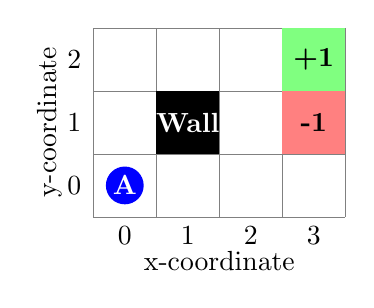
\begin{tikzpicture}[scale=0.8]
    % Grid
    \draw[step=1cm,gray,very thin] (0,0) grid (4,3);
    
    % Walls
    \fill[black] (1,1) rectangle (2,2);
    \node at (1.5,1.5) {\color{white}\textbf{Wall}};
    
    % Goal
    \fill[green!50] (3,2) rectangle (4,3);
    \node at (3.5,2.5) {\textbf{+1}};
    
    % Penalty
    \fill[red!50] (3,1) rectangle (4,2);
    \node at (3.5,1.5) {\textbf{-1}};
    
    % Starting position
    \fill[blue] (0.5,0.5) circle (0.3);
    \node at (0.5,0.5) {\color{white}\textbf{A}};
    
    % Grid labels
    \foreach \x in {0,1,2,3}
        \node at (\x+0.5,-0.3) {\x};
    \foreach \y in {0,1,2}
        \node at (-0.3,\y+0.5) {\y};
    
    \node at (2,-0.7) {x-coordinate};
    \node[rotate=90] at (-0.7,1.5) {y-coordinate};
\end{tikzpicture}
\end{center}

\subsection{State Representation}
Agent positions $(x, y)$ are encoded as one-hot vectors of length 12, where only the index corresponding to $y \times 4 + x$ is set to 1. This representation provides a clear input for the neural network.

\section{Methodology}

\subsection{Deep Q-Network Architecture}
The DQN consists of a simple fully-connected neural network:
\begin{itemize}
    \item \textbf{Input Layer:} 12 neurons (one-hot encoded state)
    \item \textbf{Hidden Layer:} 12 neurons with ReLU activation
    \item \textbf{Output Layer:} 4 neurons (Q-values for each action)
\end{itemize}

\subsection{Key DQN Components}
\textbf{1. Experience Replay:}
 Transitions $(s, a, s', r, done)$ where $s$ is the 
 current state, $a$ is the action taken, $s'$ is 
 the resulting state, $r$ is the reward,
  and $done$ indicates episode termination
   are stored in a replay buffer (capacity: 2000)
    and mini-batches of size 64 are randomly
     sampled for training. 
     This breaks correlation between 
     consecutive samples and improves learning stability.

\textbf{2. Target Network:} 
A separate target network with 
frozen parameters is used to 
compute target Q-values.
 The target network is synchronized 
 with the policy network every $10$ steps
  to reduce oscillations.

\textbf{3. Epsilon-Greedy Exploration:}
 Action selection balances exploration
  and exploitation using exponentially
   decaying epsilon:

\begin{equation}
\epsilon(t) = \epsilon_{end} + (\epsilon_{start} - \epsilon_{end}) \times e^{-0.005 \times t}
\end{equation}

where $\epsilon_{start} = 1.0$ and $\epsilon_{end} = 0.0001$.

\subsection{Loss Function and Optimization}

The network minimizes the Mean Squared Error 
between predicted Q-values and target Q-values:

\begin{equation}
L(\theta) = \mathbb{E}_{(s,a,r,s')}\left[\left(r + \gamma \max_{a'} Q(s', a'; \theta^-) - Q(s, a; \theta)\right)^2\right]
\end{equation}

where $\theta^-$ denotes target network
 parameters and $\gamma = 0.9$ is the discount factor. 
 Adam optimizer with learning rate $\alpha = 0.001$ 
 updates the policy network parameters.

\begin{algorithm}
    \caption{DQN Training Algorithm}
    \label{alg:dqn-training}
    \SetAlgoLined
    \footnotesize
    Initialize policy network $Q(s,a;\theta)$ and target network $Q(s,a;\theta^-)$\; \label{alg:initialize-networks}
    Initialize replay memory $\mathcal{D}$ with capacity 2000\; \label{alg:initialize-replay-memory}
    \For{episode = 1 to 2000 \label{alg:episodes_loop}}{
        Reset environment, $s \leftarrow (0,0)$\; \label{alg:reset-env}
        \For{step = 1 to 80 \label{alg:steps_loop}}{
            Select action $a = \begin{cases} \label{alg:select-action}
            \text{random} & \text{with prob. } \epsilon \\
            \arg\max_a Q(s,a;\theta) & \text{otherwise}
            \end{cases}$\;
            Execute $a$, observe $r, s'$, terminal flag\; \label{alg:execute-action}
            Store $(s, a, s', r, terminal)$ in $\mathcal{D}$\; \label{alg:store-transition}
            $s \leftarrow s'$\; \label{alg:update-state}
            \If{$|\mathcal{D}| > 64$}{
                Sample mini-batch of 64 from $\mathcal{D}$\; \label{alg:sample-batch}
                Compute target: $y = \begin{cases} \label{alg:compute-target}
                r & \text{if terminal} \\
                r + \gamma \max_{a'} Q(s',a';\theta^-) & \text{otherwise}
                \end{cases}$\;
                Update $\theta$ by minimizing $(y - Q(s,a;\theta))^2$\; \label{alg:update-parameters}
            }
            \If{step \% 10 == 0 \label{alg:target-sync}}{
                $\theta^- \leftarrow \theta$\; \label{alg:update-target-network}
            }
            \If{terminal \label{alg:check-terminal}}{
                break\; \label{alg:break-loop}
            }
        }
        \If{episode \% 10 == 0 \label{alg:evaluation}}{
            Evaluate policy for 10 test episodes\; \label{alg:evaluate-policy}
        }
    }
\end{algorithm}

We use Algorithm \ref{alg:dqn-training} to train the agent on the grid world environment.
We first initialize the policy and target networks along with the replay memory (lines \ref{alg:initialize-networks}-\ref{alg:initialize-replay-memory}). For each episode, we reset the environment and iterate through steps until reaching a terminal state or the maximum step limit (lines \ref{alg:reset-env}-\ref{alg:steps_loop}). Actions are selected using an epsilon-greedy strategy (line \ref{alg:select-action}), and transitions are stored in the replay buffer (line \ref{alg:store-transition}). Once enough samples are collected, we sample mini-batches to update the policy network parameters (lines \ref{alg:sample-batch}-\ref{alg:update-parameters}). The target network is synchronized every 10 steps (lines \ref{alg:target-sync}-\ref{alg:update-target-network}). 
We check if the termination condition is met (line \ref{alg:check-terminal}), i.e., if the agent reached the goal or received the penalty.
 Periodic evaluation of the policy is performed every 10 episodes (lines \ref{alg:evaluation}-\ref{alg:evaluate-policy}).

\section{Hyperparameters}

In order to ensure effective learning, 
we need to select appropriate hyperparameters.
 The chosen hyperparameters for the DQN implementation
  are summarized in Table \ref{tab:hyperparameters}.

\begin{table}[h]
\centering

\caption{DQN Hyperparameters}
\begin{tabular}{|l|c|}
\hline
\textbf{Parameter} & \textbf{Value} \\
\hline
Learning rate ($\alpha$) & 0.001 \\
Discount factor ($\gamma$) & 0.9 \\
Replay memory size & 2000 \\
Mini-batch size & 64 \\
Target network sync frequency & 10 steps \\
$\epsilon_{start}$ & 1.0 \\
$\epsilon_{end}$ & 0.0001 \\
$\epsilon$ decay rate & 0.005 \\
Training episodes & 2000 \\
Max steps per episode & 80 \\
Number of runs & 5 \\
Hidden layer neurons & 12 \\
\hline
\end{tabular}
\label{tab:hyperparameters}
\end{table}

\section{Results and Discussion}

The DQN agent was trained for 2000 episodes
 across 5 independent runs with different
  random seeds. 
  Training performance is shown in Fig. 1,
  where the rolling mean (window=10) 
  demonstrates convergence to an optimal policy.

\begin{figure}[h]
    \centering
    \includegraphics[width=0.48\textwidth]{./Fig/agent_reward_minus_1.pdf}
    \caption{Training performance over 2000 episodes
     averaged across 5 runs. The rolling mean shows
      convergence to positive cumulative rewards,
       indicating successful learning. 
       Shaded areas represent percentiles data, i.e., $25\%$ and $75\%$, while the $50\%$ percentile is represented by the solid line.}
\end{figure}

The agent successfully learns to navigate from $(0,0)$
 to the goal at $(3,2)$ while avoiding the penalty 
 at $(3,1)$ and the wall at $(1,1)$. 
 The experience replay mechanism and target network 
 stabilization prove effective in this discrete 
 state environment.
  The exponential epsilon decay ensures 
  sufficient exploration early in training 
  while transitioning to exploitation as
   the policy improves.

\section{Conclusion}
This work demonstrates successful implementation 
of DQN for a grid world navigation task
 with stochastic dynamics. 
 The combination of experience replay, 
 target networks, and epsilon-greedy exploration 
 enables stable learning despite the slip mechanics. 
\end{document}
